
\chapter{Механизм поддержания продольных вихрей}


В предыдущей главе описан метод получения модельного порыва и его основные характеристики. Механизм самоподдержания модельного порыва оказывается связан с бегущей волной, которая может быть в нем выделена. Длина бегущей волны приблизительно равна 5 радиусам трубы $R$. Автором работы было обнаружено, что при условии $5R$ периодичности вдоль трубы метод поиска решения на сепаратрисе дает точную бегущую волну. Она повторяет основные особенности бегущей волны, наблюдаемой в модельном порыве, но является стационарной в сопутствующей системе отсчета. Простота поведения найденного решения позволила выделить нелинейный механизм взаимодействия пульсаций, ответственный за формирование продольных вихрей, и в строгом виде продемонстрировать ряд особенностей движения, обеспечивающих его работу. В этой главе представлены результаты исследования найденной бегущей волны и их обобщение на модельный порыв. 



\section{Характеристики возникающей на сепаратрисе бегущей волны}

Применение метода поиска решения на сепаратрисе, описанного в разделе \ref{edge_seq}, в расчетной области небольшой протяженности при $L_x = 5$, $\Re = 2200$ позволило получить решение типа нелинейной бегущей волны. Возникающая бегущая волна повторяет особенности бегущей волны, наблюдаемой в модельном порыве, однако, в отличии от нее, является точной в том смысле, что её поле скорости строго периодично вдоль трубы и во времени. В сопутствующей системе отсчета новое решение оказывается стационарным, что делает его более доступным для исследования. Фазовая скорость найденной бегущей волны оказывается равной $c_{tw} = 0.77$ (<<traveling wave>>), что соответствует скорости перемещения бегущей волны в модельном порыве. Возможно, найденная бегущая волна была получена также в \cite{Chantry2014}, где сообщается о том, что локализованное вдоль трубы решение, соответствующее модельному порыву, порождается некоторой бегущей волной вследствие потери ей симметрии. 

Как при исследовании модельного порыва, разделим поле скорости бегущей волны $\v_{tw}$ на стационарную $\V_{tw} = \overline{\v_{tw}}^{x}$ и пульсационную $\v_{n,tw} = \v_{tw} - \V_{tw}$ составляющие. В модельном порыве осреднение выполняется по времени в сопутствующей системе отсчета, в которой бегущая волна перемещается вниз по потоку. В случае точной бегущей волны такое осреднение эквивалентно осреднению вдоль трубы, что позволяет отказаться от переменной времени. Для того, чтобы представить средние характеристики бегущей волны на иллюстрации, достаточно привести их значение только в одном сечении трубы, так как они не зависят от $x$.

Продольная и поперечная компоненты среднего поля скорости бегущей волны $\V_{tw}$, изображены на рисунке \ref{pipetw_pic},{\it a,b}. Оно повторяет среднее поле скорости модельного порыва в той области, где наблюдаются пульсации. На границах расчетной области, где быстрая жидкость проникает ближе к стенке, расположены полосы повышенной скорости, в центре расчетной области --- полоса пониженной скорости. Поперечное движение может быть ассоциировано с продольными вихрями. В расчетную область попадает пара таких вихрей, поддерживающих существование полос. Пульсационная составляющая, амплитуда которой изображена в на рисунке \ref{pipetw_pic},{\it с}, также повторяет пульсации, наблюдаемые в модельном порыве (смотри рисунок \ref{puls_cs_pic}). Пульсации сосредоточены между полосами повышенной и пониженной скорости и в системе отсчета наблюдателя представляют собой волнообразное смещение области пониженной скорости в угловом направлении. Отметим, что движение жидких частиц может не совпадать с движением области пониженной скорости. Рисунок \ref{pipetw_pic},{\it d} позволяет сравнить мгновенное поле скорости пульсационной составляющей движения для бегущей волны $\v_{n,tw}$ и для модельного порыва~$\v_n$ (смотри рисунок \ref{puls_ls_pic}). На рисунках изображена продольная компонента скорости в сечении $\theta = 0$. 
 

\begin{figure}
\center{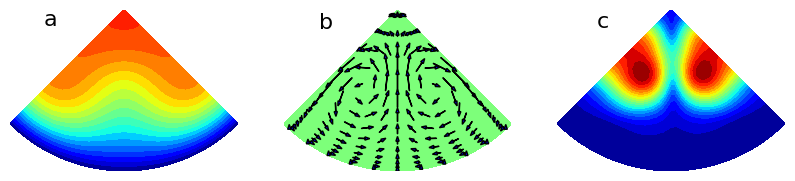
\includegraphics[width=0.9\linewidth]{pipetw_means.png}}
\center{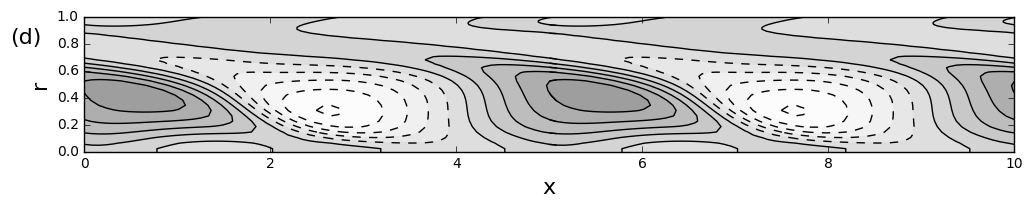
\includegraphics[width=0.9\linewidth]{pipetw_v1_ls.png}}
\caption{Поле скорости бегущей волны, возникающей на сепаратрисе: {\it a, b} --- продольная и поперечная компоненты среднего течения $\V_{tw}$, {\it c} --- амплитуда пульсаций $\v_{n,tw}$, {\it d} --- продольная компонента пульсаций в сечении $\theta = 0$.}
\label{pipetw_pic}
\end{figure}

Хотя найденная бегущая волна повторяет качественные особенности модельного порыва, наблюдаются существенные количественные отличия. Для сравнения с модельным порывом, на рисунке \ref{pipetw_amp_pic} приведена амплитуда компонент движения бегущей волны, осредненная по времени и по сечению трубы. В отличии от модельного порыва, их значение не зависит от продольной координаты. По аналогии с модельным порывом, в среднем течении $\V_{tw}$ выделена двумерная компонента $\V_{2D,tw} = \overline{\V_{tw}}^\theta$. Трехмерная составляющая движения $\V_{3D,tw} = \V_{tw} - \V_{2D,tw}$ разделена на продольную $\V_{S,tw}$ и поперечную $\V_{V,tw}$, связанные с полосами и продольными вихрями, соответственно. Качественно соотношение между интенсивностью компонент движения сохраняется, однако в модельном порыве они достигают больших значений. Наибольшее отличие демонстрирует поперечное движение $\V_V$, для бегущей волны его значение более, чем в три раза ниже наибольшего значения, достигаемого в модельном порыве. Это может объясняться тем, что решение на сепаратрисе является равновесным. Равновесная интенсивность продольных вихрей в бегущей волне обусловлена необходимостью преодоления диссипирующего влияния вязкости. В модельном порыве необходима большая интенсивность вихрей для того, чтобы не только поддерживать, но и формировать полосы в попадающем внутрь порыва ламинарном течении. 


\begin{figure}
\center{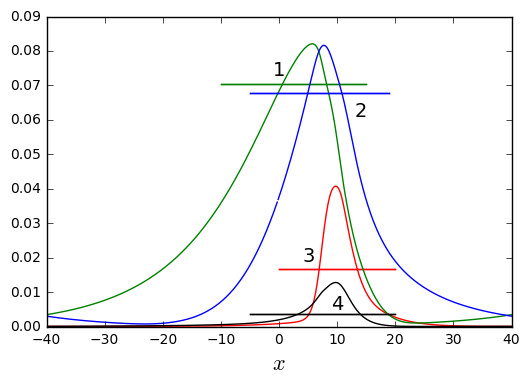
\includegraphics[width=0.5\linewidth]{pipetw_amp.png}}
\caption{Средняя по сечению трубы амплитуда компонент движения бегущей волны (горизонтальные линии) в сравнении с аналогичными величина для модельного порыва (функции переменной $x$): 1 --- движение $\V_S$, ассоциированное с полосами; 2 --- отклонение от течения Пуазейля двумерной компоненты движения $\V_{2D}$; 3 --- пульсационная составляющая движения $\v_n$; 4 --- движение $\V_V$, ассоциированное с продольными вихрями. График повторяет рисунок \ref{amp_pic}.}
\label{pipetw_amp_pic}
\end{figure}

Пульсационная составляющая движения бегущей волны $\v_{n,tw}$ возникает в результате линейной неустойчивости стационарного течения $\V_{tw}$. Наиболее быстро растущее собственное решение линеаризованного уравнения для возмущений \eqref{lin_eq} воспроизводит форму пульсационной составляющей движения и её фазовую скорость. Соответствующий инкремент нарастания $\lambda = 0.0085$. Для сравнения с пульсационной составляющей движения, поле скорости которой представлено на рисунке \ref{pipetw_pic},{\it c,d}, на рисунке \ref{pipetw_lin_pic},{\it a,b} изображены амплитуда пульсаций, возникающих в линейной задаче, и их мгновенное поле скорости в продольном сечении. Решение линейной задачи имеет более простую форму. Так как среднее течение однородно вдоль трубы и стационарно, линейное решение имеет форму бегущей волны, поле скорости которой меняется по гармоническому закону вдоль трубы и во времени. Как и в случае с модельным порывом, возникающие в рамках линейной задачи пульсации имеют дополнительную симметрию отражения относительно сечения $\theta = \pi/4$, выражаемую уравнением \eqref{dop_sym_eq}. 


\begin{figure}
\center{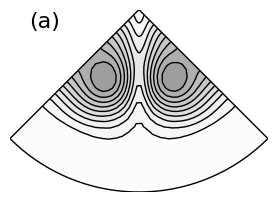
\includegraphics[width=0.3\linewidth]{pipetw_lin_amp.png} 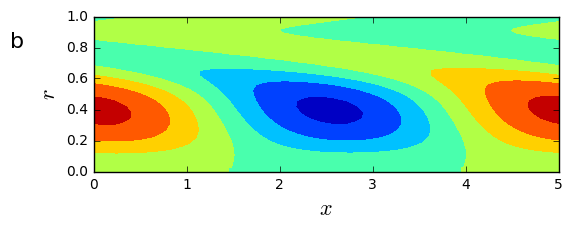
\includegraphics[width=0.6\linewidth]{pipetw_lin_ls.png}}
\caption{Наиболее быстрорастущее собственное возмущение, возникающее на среднем течении $\V_{tw}$: {\it a} --- амплитуда пульсаций, {\it b} --- продольная компонента скорости в сечении $\theta = 0$. }
\label{pipetw_lin_pic}
\end{figure}

%\lambda = - 0.0065


Возникающая на сепаратрисе бегущая волна, таким образом, воспроизводит основные элементы цикла самоподдержания модельного порыва, но имеет более простую форму. В сопутствующей системе отсчета её поле скорости оказывается стационарным. В потоке выделяются полосы повышенной и пониженной скорости. Области пониженной скорости имеют зигзагообразную форму. В системе отсчета наблюдателя движение представляет собой периодическое смещение области пониженной скорости в угловом направлении. С периодическим движением может быть ассоциирована пульсационная составляющая поля скорости. Было показано, что она возникает в результате линейной неустойчивости среднего течения, воспроизводящего полосчатый профиль скорости. Среднее течение в этом случае однородно вдоль трубы, что объясняет тот факт, что решение имеет форму бегущей волны. Также в потоке могут быть выделены стационарные продольные вихри, ответственные за образование полосчатого профиля скорости, также не меняющиеся вдоль трубы. Как будет показано далее, простота поведения бегущей волны позволяет выделить некоторые закономерности движения, справедливые также и для модельного порыва, и продемонстрировать их в строго виде. В частности, был выделен механизм нелинейного взаимодействия пульсаций, поддерживающий существование продольных вихрей. 


\section{Механизм образования продольных вихрей на примере бегущей волны}

Принято считать, что продольные вихри, ответственные за образование полос, возникают в результате некоторого нелинейного взаимодействия пульсаций, однако его детали не установлены. Прояснить процесс формирования продольных вихрей позволяет анализ уравнения, описывающего эволюцию продольной завихренности, полученного применением оператора Ротора к уравнению Навье-Стокса \eqref{NSeq_cf}:
\begin{equation}\label{ox_eq}
\pd{\omega_x}{t} - \nu\nabla^2 \omega_x =  -  (\v - \c_f, \nabla) \omega_x + (\om, \nabla) v_x
\end{equation}
Здесь $\om = (\omega_x, \omega_r, \omega_\theta) = \rot \v$ --- вектор завихренности, $\c_f$ --- скорость перемещения системы отсчета. Уравнение для стационарной составляющей продольной завихренности получается после осреднения \eqref{ox_eq} по времени в системе отсчета, связанной с порывом:
\begin{equation}\label{OX_eq}
\pd{\Omega_x}{t} - \nu\nabla^2 \Omega_x = - (\V - \c_f, \nabla) \Omega_x + (\Om, \nabla) V_x - \overline{(\v', \nabla) \omega'_x}^t + \overline{ (\om', \nabla) v'_x }^t
\end{equation}
Здесь  $\Om=(\Omega_x, \Omega_r, \Omega_\theta)$ и $\om'=(\omega'_x, \omega'_r, \omega'_\theta)$ средняя и пульсационная составляющие вектора завихренности. Отметим, что в силу линейности оператора Ротора и осреднения $\Om = \rot \V$, $\om' = \rot \v'$, где $\V$ и $\v'$ --- средняя и пульсационная составляющие поля скорости $\v$. В правой части \eqref{OX_eq} первая пара членов описывает изменение продольной завихренности за счет конвективного переноса и деформации вихревых линий осредненного течения, а вторая пара выражает порождение средней завихренности пульсационным движением. При отсутствии пульсаций продольная завихренность постепенно исчезает под действием вязкости. В рассматриваемом течении система находится в равновесии и стационарная продольная завихренность во времени не меняется. Вязкие диссипация и диффузия компенсируются генерацией завихренности членами в правой части \eqref{OX_eq}.

Для выявления определяющих механизмов генерации средней продольной завихренности удобнее рассмотреть уравнение эволюции квадрата $\Omega_x$, получающееся домножением всех членов \eqref{OX_eq} на $2\Omega_x$. Положительный или отрицательный знак у полученных таким образом выражений в правой части уравнения показывает соответственно положительный или отрицательный вклад этого члена в изменение $\Omega_x^2$, а, следовательно, и в интенсивности поперечного движения. Распределение $\Omega_x^2$ по сечению трубы представлено на рис.~\ref{OXgen_pic}(a). В большей части сечения трубы средняя продольная завихренность близка к нулю. Область концентрации $\Omega_x$ расположена между полосами повышенной и пониженной скорости вблизи области максимальной амплитуды пульсаций.

\begin{figure}
\center{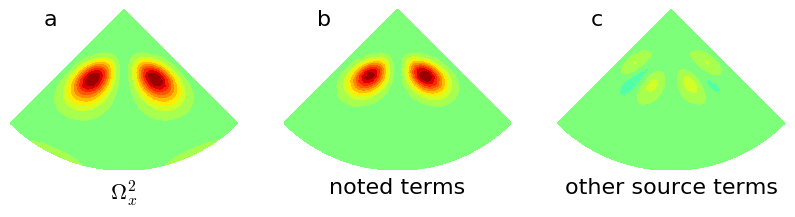
\includegraphics[width=1\linewidth]{pipetw_OXgen.png}}
\caption{Распределение по сечению трубы $\Omega_x^2$ --- (a), вклад в производство $\Omega_x^2$ слагаемых, соответствующих выделенным в \eqref{OXgen_terms} --- (b), вклад остальных слагаемых в правой части \eqref{OX_eq} --- (с). Сплошные линии соответствуют положительным значениям, прерывистые --- отрицательным.}
\label{OXgen_pic}
\end{figure}

При анализе уравнения \eqref{OX_eq} обнаружено, что два слагаемых в правой части, а именно
\begin{equation}\label{OXgen_terms}
 - \overline{v'_x \frac{\d \omega'_x}{\d x}} + \overline{ \omega'_x \frac{\d v'_x}{\d x} },
\end{equation}
вносят определяющий вклад в производство средней продольной завихренности. Соответствующее сумме \eqref{OXgen_terms}  распределение в уравнении для $\Omega_x^2$ представлено на рис.~\ref{OXgen_pic}(b), а вклад остальных слагаемых правой части \eqref{OX_eq} показан на рис.~\ref{OXgen_pic}(c). Распределение генерации $\Omega_x^2$ выделенными в \eqref{OXgen_terms} членами практически совпадает по форме с распределением $\Omega_x^2$, тогда как вклад остальных членов не имеет выраженного распределения и на порядок уступает по суммарному вкладу в генерацию $\Omega_x^2$. Таким образом, нет сомнения в том, что стационарные продольные вихри возникают в основном за счет действия выделенной в \eqref{OXgen_terms} пары слагаемых.

Отметим, что пульсации, соответствующие старшей собственной функции линейной задачи об устойчивости среднего стационарного течения, также демонстрируют приведенный выше механизм образования стационарных продольных вихрей. Важно, что это наблюдается только в том случае, когда при анализе устойчивости учитываются как продольная, так и поперечная составляющие среднего течения. Принято считать, что поперечное движение, определяя угловую неоднородность в распределении продольной скорости среднего течения, не может существенным образом влиять на свойства его устойчивости вследствие незначительности своей амплитуды. Поэтому при исследовании линейной устойчивости подобных течений, например, полосчатых структур в турбулентных потоках, наличие поперечного движения обычно не принимается во внимание. В нашем случае пренебрежение поперечным движением приводит к тому, что стационарное течение оказывается линейно устойчивым. Что еще более важно, наименее затухающее возмущение не воспроизводит при этом описанный механизм формирования продольных вихрей. Это связанно с тем, что форма пульсаций продольной завихренности $\omega'_x$ качественно меняется, хотя пульсации продольной скорости $v'_x$ сохраняют свою форму практически неизменной. Тем самым нарушается согласованность  $v'_x$ и $\omega'_x$, необходимая для обеспечения нужного вклада выражения \eqref{OXgen_terms} в производство продольной завихренности.

\begin{figure}
\center{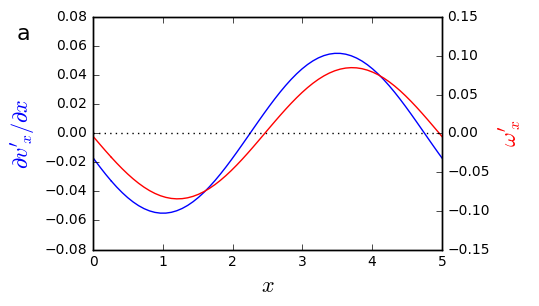
\includegraphics[width=0.5\linewidth]{pipetw_lin_cor.png}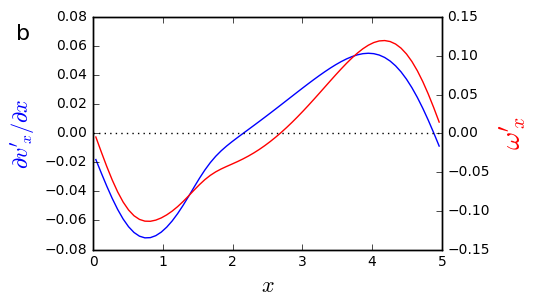
\includegraphics[width=0.5\linewidth]{pipetw_puls_cor.png}}
\caption{Распределение по сечению трубы $\Omega_x^2$ --- (a), вклад в производство $\Omega_x^2$ слагаемых, соответствующих выделенным в \eqref{OXgen_terms} --- (b), вклад остальных слагаемых в правой части \eqref{OX_eq} --- (с). Сплошные линии соответствуют положительным значениям, прерывистые --- отрицательным.}
\label{OXgen_pic}
\end{figure}


Каждое из двух слагаемых в \eqref{OXgen_terms} дает примерно половину общего вклада в производство средней продольной завихренности. Для пульсаций, полученных в рамках линеаризованной постановки, слагаемые \eqref{OXgen_terms} равны друг другу точно. Так как среднее поле скорости $\V_{tw}$ однородно вдоль трубы, возникающие на нем вследствие линейной потери устойчивости собственные возмущения меняются вдоль трубы по гармоническом закону. При фиксированных значениях $r, \theta$ пусть $v'_x = a \sin(\alpha x + \phi)$, $\omega_x' = b \sin(\alpha x + \psi)$. Тогда 
\begin{multline}
 - \overline{v'_x \frac{\d \omega'_x}{\d x}}^x + \overline{\omega'_x \frac{\d v'_x}{\d x}}^x = 
- \overline{\alpha a b \sin(\alpha x + \phi) \cos(\alpha x + \psi)}^x + \\ +
\overline{\alpha a b \cos(\alpha x + \phi) \sin(\alpha x + \psi)}^x = \alpha a b \sin(\psi - \phi).
\end{multline}
Осреднение вдоль трубы может быть опущено, слагаемые иметь равные значения 

Это значит, в частности, что колебания $\d v'_x/\d x$ и $\omega'_x$ положительно коррелированы в области концентрации положительной $\Omega_x$ и отрицательно коррелированы в области концентрации отрицательной $\Omega_x$. То же относится и к колебаниям $-v'_x$ и $\d \omega'_x/\d x$. Расчет соответствующих коэффициентов корреляции показывает, что они близки к $\pm1$ в соответствующих областях. 


\section{Механизм возникновения пульсаций продольной завихренности}

Для выявления механизма формирования такой связи между пульсациями продольных компонент скорости и завихренности рассмотрим уравнение эволюции $\omega'_x$, получающееся вычитанием \eqref{OX_eq} из \eqref{ox_eq}:
\begin{multline}\label{ox1_eq}
\pd{\omega'_x}{t} - \nu \nabla^2 \omega'_x = - (\V - \c, \nabla) \omega'_x - (\v', \nabla) \Omega_x
+(\Om, \nabla) v'_x + (\om', \nabla) V_x -\\- (\v', \nabla) \omega'_x  + (\om', \nabla) v'_x  + \overline{(\v', \nabla) \omega'_x)}  - \overline{(\om', \nabla)}
\end{multline}
Работать удобнее с уравнением, описывающим изменение среднего квадрата пульсаций продольной завихренности $\overline{\omega'^2_x}$, получающимся умножением на $2\omega'_x$ каждого из слагаемых в \eqref{ox1_eq} и последующим осреднением по времени. Как и раньше, осреднение по времени производится в подвижной системе отсчета. Слагаемые в этом уравнении не зависят от времени, сумма слагаемых в правой части балансируется вязким членом в левой части. Как и в предыдущем случае, среди всех слагаемых правой части удается выделить существенные, ответственные за возникновение пульсаций $\omega'_x$.


Распределение $\overline{\omega'^2_x}$ по сечению трубы с максимальным уровнем пульсаций изображено на рис.~\ref{ox1gen_pic}(a). Основные пульсации $\omega'_x$ наблюдаются в центре расчетной области около оси трубы. На месте расположения продольных вихрей также присутствуют пульсации $\omega'_x$, но меньшей интенсивности. В остальной части трубы их амплитуда близка к нулю. Обнаружено, что за генерацию пульсаций $\omega'_x$ в центральной части трубы и на месте продольных вихрей отвечают два разных механизма. Первый дает пульсации большей амплитуды, однако, за возникновение стационарных продольных вихрей ответственны пульсации, производимые вторым механизмом, так как именно они оказываются согласованными с пульсациями $v'_x$ нужным образом.


\begin{figure}[h]
\center{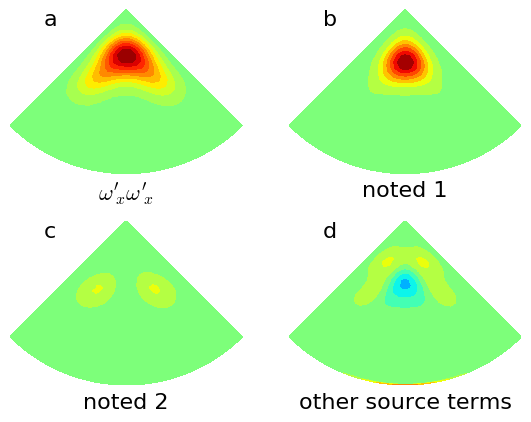
\includegraphics[width=0.66\linewidth]{pipetw_ox1gen.png}}
\caption{Распределение среднего квадрата пульсаций продольной завихренности --- а, вклад в производство $\left<\omega'^2_x \right>$ слагаемых \eqref{ox1gen_add_terms} --- (b), слагаемого \eqref{ox1gen_main_terms} --- (c) и суммы остальных слагаемых правой части \eqref{ox1_eq} --- (d).}
\label{ox1gen_pic}
\end{figure}


Первый механизм формирования $\omega'_x$ связан с наличием нормальных к стенке вихрей в пульсационной составляющей движения. Можно провести аналогию между неустойчивостью, возникающей на полосе замедления, и неустойчивостью в следе за телом. Пульсационная составляющая движения напоминает дорожку Кармана. В ней можно выделить последовательность нормальных к стенке вихрей чередующегося знака, двигающихся вниз по полосе пониженной скорости. Им соответствуют области повышенной амплитуды пульсаций радиальной завихренности $\omega'_r$. Между полосой замедления и осью трубы имеется значительный радиальный градиент продольной скорости $\d V_x/ \d r$. В его присутствии нормальные к стенке вихри поворачиваются так, что приобретают продольную составляющую $\omega'_x$. Кроме того, наличие радиального градиента $\d V_x/ \d r$ связано с наличием угловой завихренности $\Omega_\theta = \d V_r / \d x - \d V_x / \d r$. Радиальная пульсационная завихренность $\omega'_r = \d v'_x / r \d \theta - \d v'_\theta / \d x$ за счет первого из слагаемых поворачивает стационарные угловые вихри так, что те также приобретают пульсационную продольную составляющую. В уравнении \eqref{ox1_eq} за описанный механизм отвечают слагаемые:
\begin{equation}\label{ox1gen_add_terms}
\frac{\d \omega'_x}{\d t} = \omega'_r \frac {\d V_x}{\d r} +
\frac{\Omega_\theta}{r} \frac{\d v'_x}{\d \theta} + ...
\end{equation}
Несмотря на то, что выделенные в \eqref{ox1gen_add_terms} слагаемые имеют противоположные знаки и в значительной степени компенсируют друг друга при сложении, их вклад в производство $\omega'_x$ значителен (см. рис.~\ref{ox1gen_pic}(b)). Они определяют форму пульсаций $\omega'_x$ в области между полосой замедления и осью трубы, где пульсации $\omega'_x$ достигают наибольшего значения. Эти пульсации, однако, практически не участвуют в образовании стационарной составляющей продольной завихренности. Это объясняется тем, что колебания $\omega'_x$, рождающиеся в результате описанного механизма, близки по фазе к колебаниям $v'_x$, так что сомножители каждого из слагаемых в выражении \eqref{OXgen_terms} оказываются в противофазе и при осреднении дают близкие к нулю значения.


Второй механизм образования пульсаций продольной завихренности $\omega'_x$ связан с перераспределением уже существующей стационарной продольной завихренности $\Omega_x$ за счет пульсационной составляющей продольной скорости $v'_x$ (эффект сжатия/растяжения вихревых линий). В уравнении \eqref{ox1_eq} за описываемый механизм отвечает слагаемое
\begin{equation}\label{ox1gen_main_terms}
\frac{\d \omega'_x}{\d t} = \Omega_x \frac {\d v'_x}{\d x} + ...
\end{equation}
Выделенное в \eqref{ox1gen_main_terms} слагаемое стремится произвести пульсации $\omega'_x$, пропорциональные $\d v'_x / \d x$, что обеспечивает наибольшую эффективность образования $\Omega_x$ посредством их нелинейного взаимодействия. Важно, что коэффициентом пропорциональности в \eqref{ox1gen_main_terms} выступает значение средней продольной завихренности, таким образом, механизм включается именно в областях концентрации $\Omega_x$. При этом производимые пульсации $\omega'_x$ положительно пропорциональны пульсациям  $\d v'_x / \d x$ при $\Omega_x>0$ и отрицательно пропорциональны при $\Omega_x<0$, что обеспечивает максимально возможную эффективность производства средней продольной завихренности нужного знака посредством второго из слагаемых выражения \eqref{OXgen_terms}. Очевидно, что пульсации $-v'_x$ и $\d \omega'_x / \d x$ в этом случае также согласованы нужным образом, так что первое слагаемое \eqref{OXgen_terms} близко по значению ко второму.


На рис.~\ref{ox1gen_pic}(c) приведен вклад выделенного в \eqref{ox1gen_main_terms} слагаемого в производство $\overline{\omega'^2_x}$. Нет сомнения, что именно это слагаемое определяет форму пульсаций в области существования продольных вихрей между полосами повышенной и пониженной скорости. Суммарный вклад других слагаемых правой части \eqref{ox1_eq}, не попавших на рис.~\ref{ox1gen_pic}(b,c), изображен на рис.~\ref{ox1gen_pic}(d). Эти слагаемые не имеют существенного значения в процессе генерации $\omega'_x$, их суммарный вклад не превышает нескольких процентов.

Описанный механизм генерации пульсаций продольной завихренности проявляется в области, где фазовая скорость волны, соответствующей пульсационной составляющей течения, близка по значению к локальной продольной скорости среднего течения. На удалении от точки генерации пульсаций, где фазовая скорость волны существенно отличается от средней скорости, выделенный в \eqref{ox1gen_main_terms} механизм генерации $\omega'_x$ практически не работает. Это объясняется тем, что в системе отсчета, связанной с волной, образующаяся посредством механизма \eqref{ox1gen_main_terms} $\omega'_x$ сносится вдоль трубы средним течением. При этом теряется согласованность фаз между $\d v'_x / \d x$ и $\omega'_x$, что делает её рост невозможным.


Описанный механизм генерации пульсаций продольной завихренности объясняет необходимость учета поперечного движения при исследовании устойчивости стационарного течения. Пренебрежение связанной с поперечным движением $\Omega_x$ делает невозможным генерацию $\omega'_x$ в форме, необходимой для сохранения поперечного движения, а следовательно и всего процесса самоподдержания пульсаций.


\section{Обобщение полученных при исследовании бегущей волны результатов на модельный порыв}

\section{Необходимость учета поперечной компоненты стационарного течения для адекватного воспроизведения формы пульсаций}

Отметим, что пульсации, соответствующие старшей собственной функции линейной задачи об устойчивости среднего стационарного течения, также демонстрируют приведенный выше механизм образования стационарных продольных вихрей. Важно, что это наблюдается только в том случае, когда при анализе устойчивости учитываются как продольная, так и поперечная составляющие среднего течения. Принято считать, что поперечное движение, определяя угловую неоднородность в распределении продольной скорости среднего течения, не может существенным образом влиять на свойства его устойчивости вследствие незначительности своей амплитуды. Поэтому при исследовании линейной устойчивости подобных течений, например, полосчатых структур в турбулентных потоках, наличие поперечного движения обычно не принимается во внимание. В нашем случае пренебрежение поперечным движением приводит к тому, что стационарное течение оказывается линейно устойчивым. Что еще более важно, наименее затухающее возмущение не воспроизводит при этом описанный механизм формирования продольных вихрей. Это связанно с тем, что форма пульсаций продольной завихренности $\omega'_x$ качественно меняется, хотя пульсации продольной скорости $v'_x$ сохраняют свою форму практически неизменной. Тем самым нарушается согласованность  $v'_x$ и $\omega'_x$, необходимая для обеспечения нужного вклада выражения \eqref{OXgen_terms} в производство продольной завихренности.


